\documentclass[11pt]{article}\usepackage[]{graphicx}\usepackage[]{color}
% maxwidth is the original width if it is less than linewidth
% otherwise use linewidth (to make sure the graphics do not exceed the margin)
\makeatletter
\def\maxwidth{ %
  \ifdim\Gin@nat@width>\linewidth
    \linewidth
  \else
    \Gin@nat@width
  \fi
}
\makeatother

\definecolor{fgcolor}{rgb}{0.345, 0.345, 0.345}
\newcommand{\hlnum}[1]{\textcolor[rgb]{0.686,0.059,0.569}{#1}}%
\newcommand{\hlstr}[1]{\textcolor[rgb]{0.192,0.494,0.8}{#1}}%
\newcommand{\hlcom}[1]{\textcolor[rgb]{0.678,0.584,0.686}{\textit{#1}}}%
\newcommand{\hlopt}[1]{\textcolor[rgb]{0,0,0}{#1}}%
\newcommand{\hlstd}[1]{\textcolor[rgb]{0.345,0.345,0.345}{#1}}%
\newcommand{\hlkwa}[1]{\textcolor[rgb]{0.161,0.373,0.58}{\textbf{#1}}}%
\newcommand{\hlkwb}[1]{\textcolor[rgb]{0.69,0.353,0.396}{#1}}%
\newcommand{\hlkwc}[1]{\textcolor[rgb]{0.333,0.667,0.333}{#1}}%
\newcommand{\hlkwd}[1]{\textcolor[rgb]{0.737,0.353,0.396}{\textbf{#1}}}%
\let\hlipl\hlkwb

\usepackage{framed}
\makeatletter
\newenvironment{kframe}{%
 \def\at@end@of@kframe{}%
 \ifinner\ifhmode%
  \def\at@end@of@kframe{\end{minipage}}%
  \begin{minipage}{\columnwidth}%
 \fi\fi%
 \def\FrameCommand##1{\hskip\@totalleftmargin \hskip-\fboxsep
 \colorbox{shadecolor}{##1}\hskip-\fboxsep
     % There is no \\@totalrightmargin, so:
     \hskip-\linewidth \hskip-\@totalleftmargin \hskip\columnwidth}%
 \MakeFramed {\advance\hsize-\width
   \@totalleftmargin\z@ \linewidth\hsize
   \@setminipage}}%
 {\par\unskip\endMakeFramed%
 \at@end@of@kframe}
\makeatother

\definecolor{shadecolor}{rgb}{.97, .97, .97}
\definecolor{messagecolor}{rgb}{0, 0, 0}
\definecolor{warningcolor}{rgb}{1, 0, 1}
\definecolor{errorcolor}{rgb}{1, 0, 0}
\newenvironment{knitrout}{}{} % an empty environment to be redefined in TeX

\usepackage{alltt}
\usepackage{amsmath}
\usepackage{amssymb}
\usepackage{geometry}
\usepackage{graphicx}
\usepackage{fullpage}
\usepackage{enumerate}
\IfFileExists{upquote.sty}{\usepackage{upquote}}{}
\begin{document}
\setlength\parindent{0pt}




Lecture 12: Simple Linear Regression\\
Practice Problems\\
STAT 310, Spring 2021\\

The following scatterplot shows the association between price (in \$1,000's) and mileage (number of miles driven in 1,000's) for a sample of 30 used Honda Accords in 2017.  Also provided below is the output from fitting a simple linear regression model in R.\\

\begin{figure}[ht]
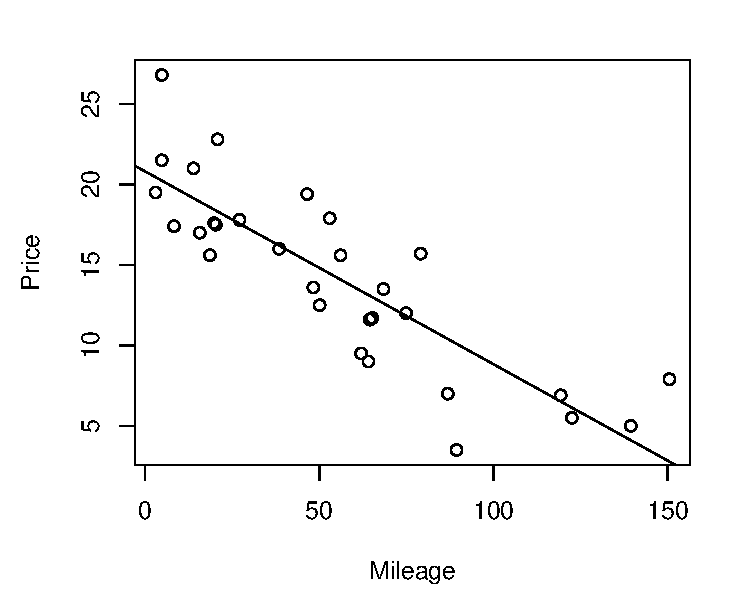
\includegraphics[scale=0.75]{figure/scatter_cars.pdf}
\end{figure}

\begin{verbatim}
Coefficients:
            Estimate Std. Error t value Pr(>|t|)    
(Intercept)  20.8096     0.9529   21.84  < 2e-16 ***
Mileage      -0.1198     0.0141   -8.50 3.06e-09 ***
---
Signif. codes:  0 ‘***’ 0.001 ‘**’ 0.01 ‘*’ 0.05 ‘.’ 0.1 ‘ ’ 1

Residual standard error: 3.085 on 28 degrees of freedom
Multiple R-squared:  0.7207,	Adjusted R-squared:  0.7107 
F-statistic: 72.25 on 1 and 28 DF,  p-value: 3.055e-09
\end{verbatim}
\vspace{2pt}

\begin{enumerate}[(a)]
\item Describe the association between price and mileage.\\
\vspace{0.75cm}

\item What are the explanatory and response variables for the linear regression model?\\
\vspace{1.5cm}

\item Write the equation for the least squares line.\\
\vspace{1.5cm}

\item What is the predicted price for a used Honda Accord that has been driven 50 thousand miles?\\ 
\vspace{1.5cm}

\item Interpret the slope.\\
\vspace{3cm}

\item Interpret the intercept.\\
\vspace{3cm}

\item Calculate the residual for a car, in this data set, that costs 3.5 thousand dollars, and has been driven 89.4 thousand miles.\\ 
\vspace{3cm}

\item Interpret the R$^2$.\\
\end{enumerate}


\end{document}
